\section{Memory}
A memory unit is a device to which binary information is transferred for storage and from which information is retrieved when needed for processing. A memory unit is an integral part of any computing system, and its primary purpose is to hold instructions and data. When data processing takes place, information from memory is transferred to selected registers in the processing unit. Intermediate and final results obtained in the processing unit are transferred back to be
stored in memory.

\par \figref{ModernComputer} shows a logical picture of components of a Modern Computer. One can observe how different types of memories are interfaced with a processor.

\begin{figure}[H]
	\begin{center}
		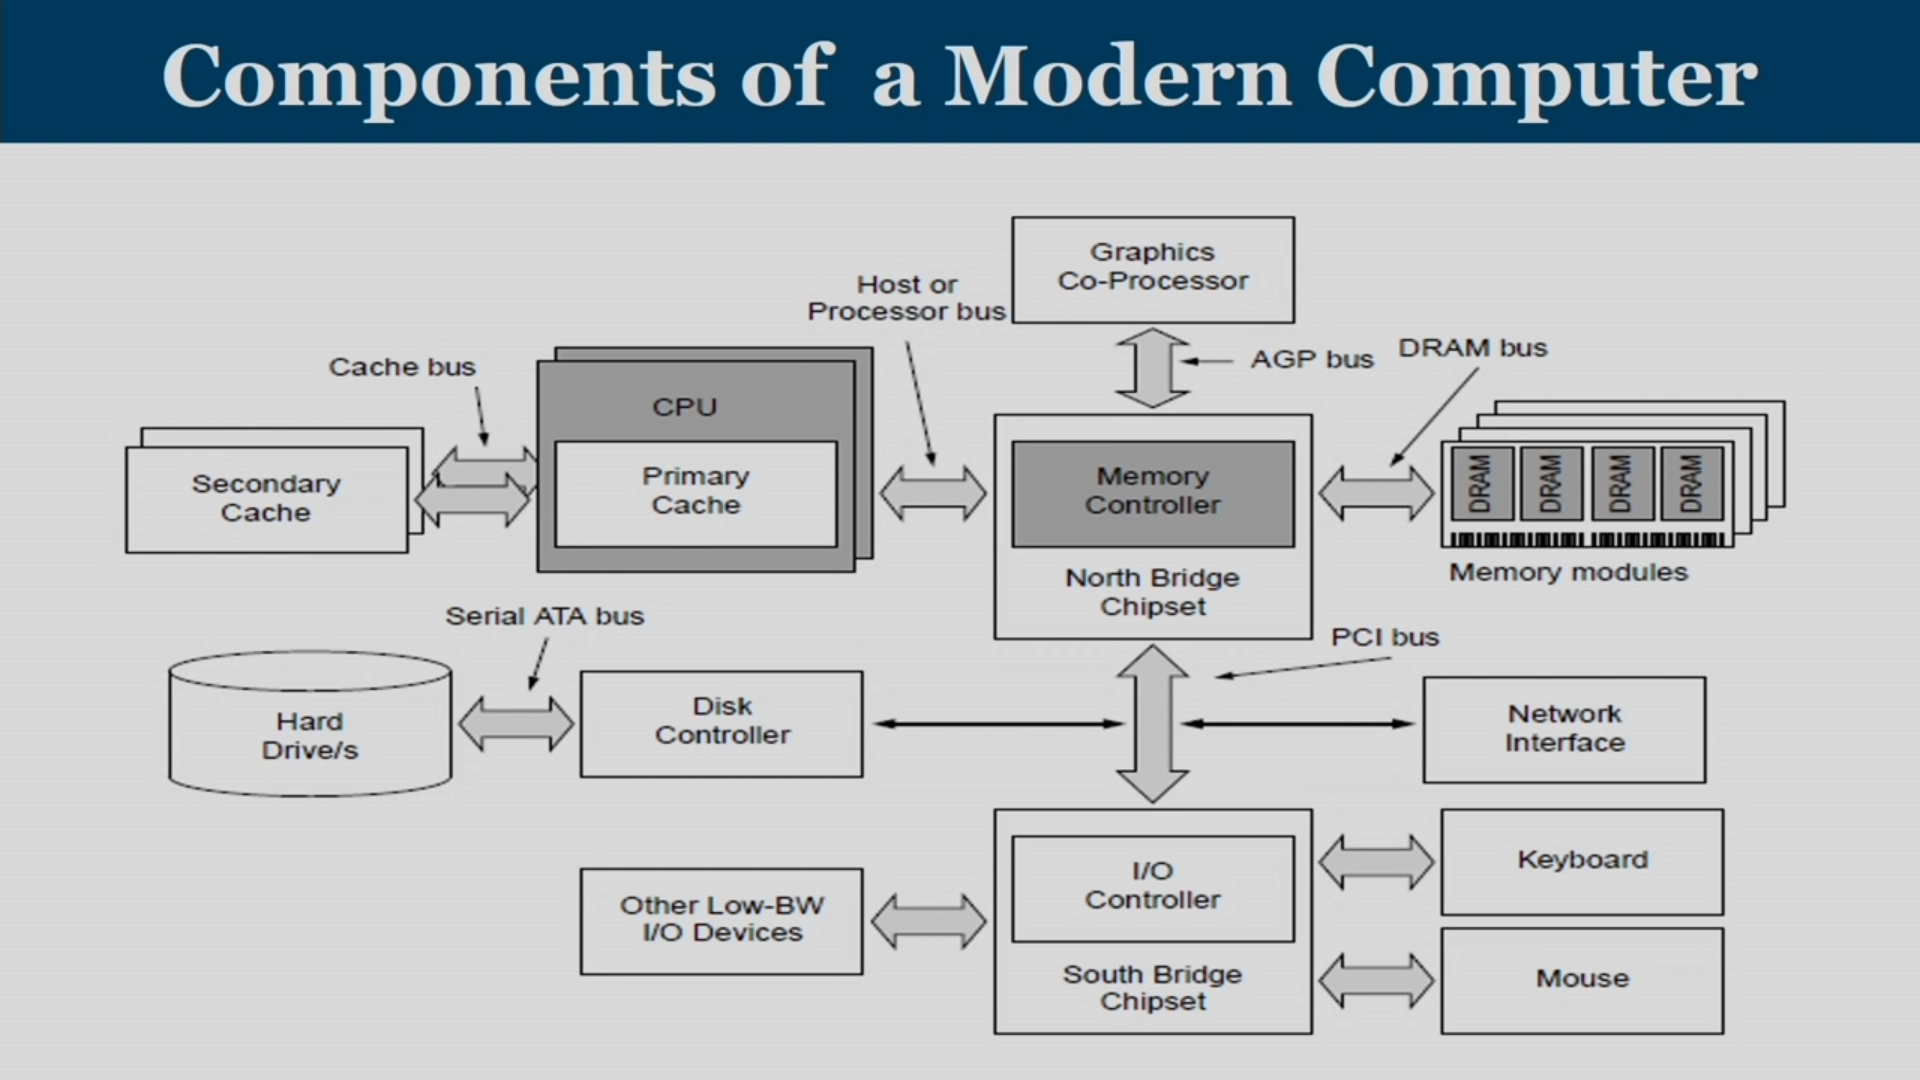
\includegraphics[width=\textwidth]{images/ModernComputer.png}
		\caption{Component of a Modern Computer}
		\label{ModernComputer}
	\end{center}
\end{figure}


\subsection{Types of memory}
In a broad sense, a memory system in any digital systems can be divided into two types:
\begin{enumerate}
    \item Read Only Memory (ROM), and
    \item Random Access Memory (RAM)
\end{enumerate}
 
\textbf{Read Only Memory (ROM)} is a type of memory where the data has been prerecorded. This means that suitable binary information is already stored inside memory and can be retrieved or read at any time. However, that information cannot be altered by writing. Data stored in ROM is retained even after the computer is turned off \ie non-volatile. There are four types of ROM:
\begin{description}
    \item[Programmable ROM (PROM)] where the data is written after the memory chip has been created. It is non-volatile.
    \item[Erasable Programmable ROM (EPROM)] where the data on this non-volatile memory chip can be erased by exposing it to high-intensity UV light.
    \item[Electrically Erasable Programmable ROM (EEPROM)] where the data on this non-volatile memory chip can be electrically erased using field electron emission.
    \item[Mask ROM] in which the data is written during the manufacturing of the memory chip.
\end{description}

\par \textbf{Random Access Memory (RAM)} is used to store the programs and data being used by the CPU in real-time. The data on the random access memory can be read, written, and erased any number of times. RAM is a hardware element where the data being currently used is stored. It is a volatile memory which means that the data stored on the RAM gets erased on a power reset. 

\subsection{Memory Hierarchy Design}
In the Computer System Design, Memory Hierarchy is an enhancement to organize the memory such that it can minimize the access time. The Memory Hierarchy was developed based on a program behavior known as locality of references. \figref{MemoryStructure} clearly demonstrates the different levels of memory hierarchy:

\begin{figure}[H]
	\begin{center}
		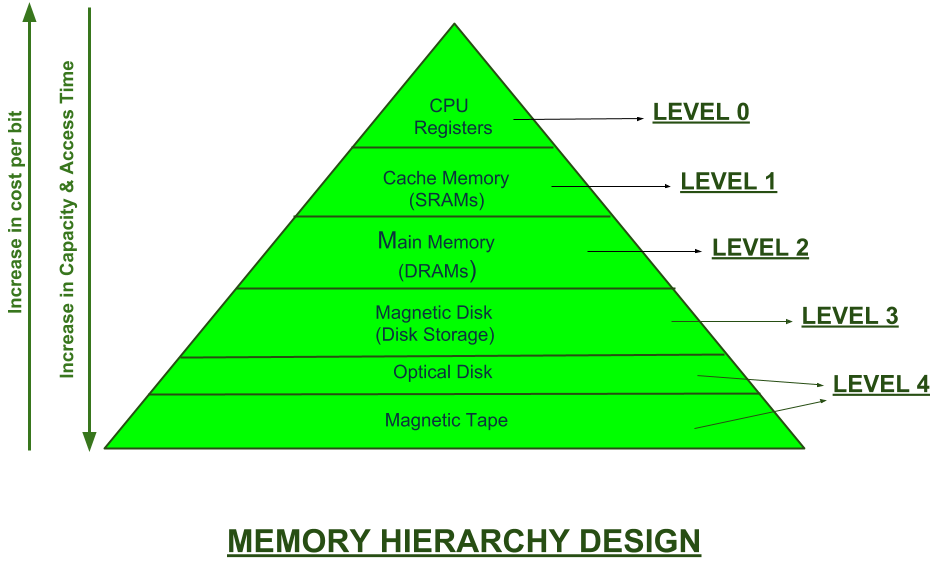
\includegraphics[width=\textwidth]{images/MemoryStructure.png}
		\caption{Component of a Modern Computer}
		\label{MemoryStructure}
	\end{center}
\end{figure}

This Memory Hierarchy Design is divided into 2 main types:
\begin{description}
    \item[External Memory or Secondary Memory] Comprising of Magnetic Disk, Optical Disk, Magnetic Tape \ie peripheral storage devices which are accessible by the processor via I/O Module.
    \item[Internal Memory or Primary Memory] Comprising of Main Memory, Cache Memory \& CPU registers. This is directly accessible by the processor.
\end{description}

In the Internal Memory or Primary Memory, the entire program and data of a given application cannot be located fully inside local memories \eg BRAMs, UltraRAMs(FPGAs), cache memories (processors). The memory is implemented as a hierarchy, where we have the registers inside the processor/FPGAs as the fastest memory, then we have caches/BRAMs. And, then the next level of memory is known as the main memory or DRAM system. 